\subsection{Concordia Contracts Provider} \label{subsection:4-3-5-concordia-contracts-provider-service}

\subsubsection{Περιγραφή - Στόχοι υπηρεσίας}

Η υπηρεσία Contracts Provider αποτελεί μία βοηθητική υπηρεσία η οποία υλοποιεί ένα απλό αποθετήριο για τα \textenglish{contract artifact}. Είναι γραμμένη σε JavaScript και διαθέτει δύο HTTP \textenglish{endpoint}, ένα για τη μεταφόρτωση (upload) των artifact προς την υπηρεσία και ένα για τη λήψη (download) από την υπηρεσία. Η υπηρεσία υποστηρίζει επίσης την επισύναψη ετικετών στα artifact, όπως της έκδοσης (version) ή του κλαδιού ανάπτυξης (για παράδειγμα \textenglish{master/develop}). Η αρχιτεκτονική της φαίνεται στο σχήμα \ref{figure:4-3-concordia-contracts-provider-architecture}.

\vspace{.5\baselineskip}

\begin{figure}[H]
    \centering
    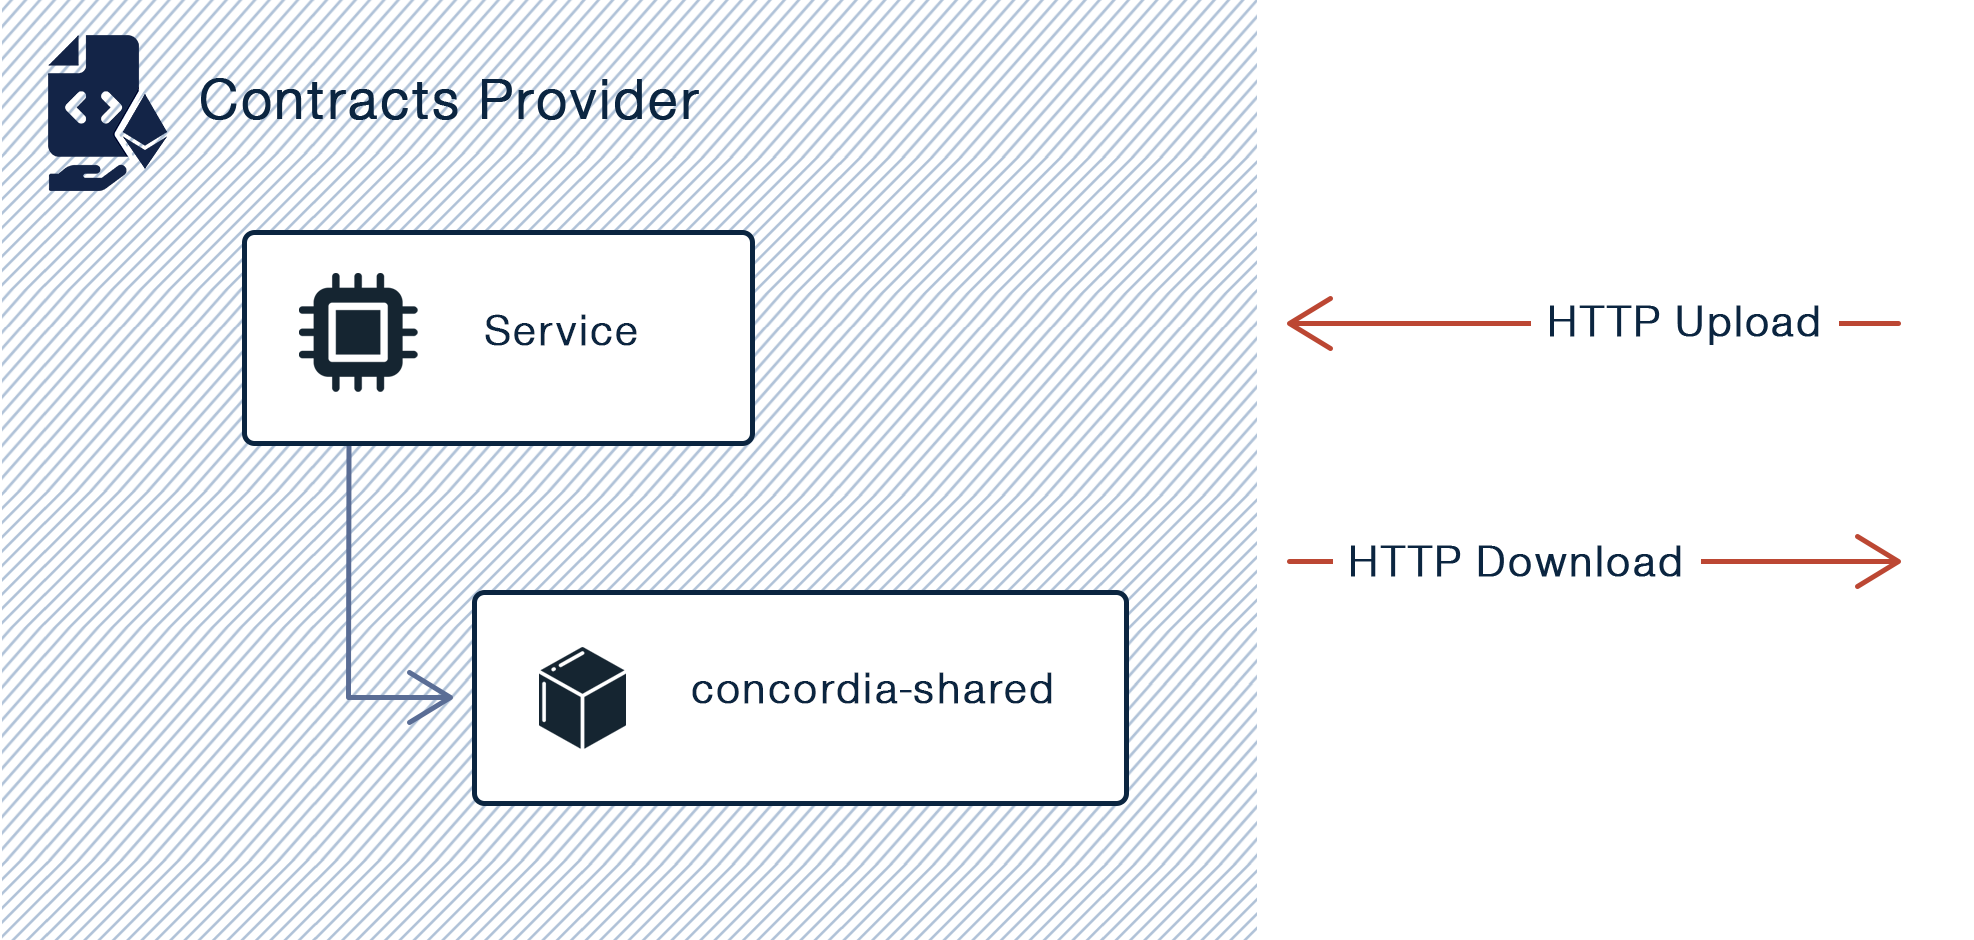
\includegraphics[width=.75\textwidth]{assets/figures/chapter-4/4.3.architecture-4.3.5.concordia-contracts-provider-architecture}
    \caption{Αρχιτεκτονική υπηρεσίας Concordia Contracts Provider}
    \label{figure:4-3-concordia-contracts-provider-architecture}
\end{figure}

Αυτή η υπηρεσία χρησιμοποιείται σε μία προσπάθεια αποσυσχέτισης της βασικής εφαρμογής που υλοποιεί η υπηρεσία Concordia Application από μία συγκεκριμένη έκδοση των contract. Οι λόγοι που αυτό είναι επιθυμητό αναπτύχθηκαν στην περιγραφή της υπηρεσίας Concordia \textenglish{Application} (υποενότητα \ref{subsection:4-3-2-concordia-application-service}). Ωστόσο, η υπηρεσία Contracts Provider αποτελεί σημείο κεντροποίησης του συστήματος και για αυτόν τον λόγο θεωρείται προσωρινή λύση για τη διευκόλυνση της προγραμματιστικής διαδικασίας. Για τη χρήση της εφαρμογής σε production, μπορεί να αντικατασταθεί με αποκεντρωτικές λύσεις, όπως με τη μεταφόρτωση και τον διαμοιρασμό των artifact μέσω του IPFS.

\subsubsection{Διανομή}

Η υπηρεσία γίνεται διαθέσιμη για χρήση ως Docker image μέσω του αποθετηρίου εικόνων Docker Hub\footnote{\url{https://hub.docker.com/r/ecentrics/concordia-contracts-provider}}. Οι χρήστες μπορούν, χρησιμοποιώντας μεταβλητές περιβάλλοντος, να αλλάξουν παραμέτρους της εκτέλεσης, όπως τη διαδρομή αποθήκευσης των μεταφορτωμένων \textenglish{contract artifact}.